\section{引言}
\subsection{绪论}
随着城市化建设的开展,我国对高层建筑的需求逐步增加。由于风载、地震等外界激励,高层建筑的振动不可避免。如何高效而经济地控制高层建筑的振动仍然困扰着工程界。本文将利用磁流变液构建基于能量收割的半主动控制磁流变阻尼系统。

本章将介绍结构振动控制问题研究现状与磁流变液及磁流变阻尼器。第二章将介绍基于能量收割的半主动控制磁流变阻尼器实现原理,主要包括振动能量收割原理、半主动控制算法、实验模型设计,并概述该系统相比现行结构控制体系的优势与创新。第三章将介绍目前的实验进展,主要包括MR阻尼器设计、力学性质测试、半主动控制系统搭建及用于收割能量的发电系统设计。

\subsection{结构振动控制问题研究现状}
1972年,Yao最初提出土木工程结构振动控制的概念\cite{yao1972concept}。其基本思想是在结构中安装特定的控制装置,对结构施加控制力或调整动力性能。经过近半个世纪的发展,从外界能量输入的角度可以将结构振动控制分为被动控制、主动控制和半主动控制三种。

\subsubsection{被动控制}
被动控制利用隔震、减震装置隔离、吸收振动,保护主体结构,防止振动在结构中传播。被动控制系统构造简单、不依赖于外界供能,主要可分为基础隔震、耗能减震和调谐减震三种方式。
\begin{enumerate}[leftmargin=*,labelindent=16pt,label=\bfseries \arabic*.]
	\item 基础隔震最早由日本学者河合浩藏于1881年提出,指在建筑物或构筑物基底设置夹层,阻止地震能量向基础以上传播。基础隔震不仅适用于一般的多层建筑,也已成功应用于桥梁的振动控制。但是,基础隔震控制效果有限,无法适应高层建筑的抗震需求\cite{Sun2012}。
	\item 耗能隔震系统将阻尼等耗能吸震装置设置在结构的节点等连接处,在外界激励下,耗能装置首先进入弹性甚至非弹性状态,发生较大变形,大量吸收外力能量,保护主体结构。耗能装置便于维护、更换,性能发挥稳定,但对一栋大型建筑而言,耗能装置体量显著提升,成本较高。
	\item 调谐减震系统增设局部的子结构,通过子结构与主体结构之间的刚度、自振周期及质量之间的关系减小主体结构振幅,将振动能量转移给子结构。这也是目前广泛采用的动力吸振器的原理。

\end{enumerate}

	假设一双自由度体系,在动力荷载作用下的振动方程为:
	\begin{equation}
	\label{vibration}
	\left\{
	\begin{array}{rl}
	m_1\ddot{y_1}\left(t\right)+k_{11}y_1\left(t\right)+k_{12}y_2\left(t\right)&=F_{P1}\left(t\right)\\
	m_2\ddot{y_2}\left(t\right)+k_{21}y_1\left(t\right)+k_{22}y_2\left(t\right)&=F_{P2}\left(t\right)
	\end{array}
	\right.
	\end{equation}
	假设外界激励为简谐荷载,即:
	\begin{equation}
	\label{sin}
	\left\{
	\begin{array}{rl}
	F_{P1}\left(t\right)&=F_{P1}\sin \theta t\\
	F_{P2}\left(t\right)&=F_{P2}\sin \theta t
	\end{array}
	\right.
	\end{equation}
	在平稳振动阶段,各质点也将做简谐振动,即:
	\begin{equation}
	\label{sinMove}
	\left\{
	\begin{array}{rl}
	y_{1}\left(t\right)=Y_{1}\sin \theta t\\
	y_{2}\left(t\right)=Y_{2}\sin \theta t
	\end{array}
	\right.
	\end{equation}
	
	最终可解得:
	\begin{equation}
	\label{answer}
	\left\{
	\begin{array}{rl}
	D_0&=\left(k_{11}-\theta^2m_1\right)\left(k_{22}-\theta^2m_2\right)-k_{12}k_{21} \\
	D_1&=\left(k_{22}-\theta^2m_2\right)F_{P1}-k_{12}F_{P2} \\
	D_2&=-k_{21}F_{P1}+\left(k_{11}-\theta^2m_1\right)F_{P2}
	\end{array}
	\right.
	\end{equation}
	
	当$F_2=0$,$k_2=\theta^2m_2$时,由式\eqref{answer}可知$D_0=k_2^2$,且$Y_1=0$,$Y_2=-\frac{F_p}{k_2}$,即增加子结构$m_2$后,主结构$m_1$的振动被消除。
	
	从上述求解过程也可以看出,调谐减震系统由于事先需要确定减震所需的子结构刚度、质量等条件,可调节范围窄。当外界激励离设计值偏差较大时,抗震效果不能令人满意。
	
	下图就展示了一个由单自由度振子和其下方的动力吸振器组成的振动系统。对于这样一个系统,激振频率与主体结构的振幅的关系由下图中的曲线描述,可以看到,只有在外界激振力的频率处于一个很小的范围(图上阴影区域)时,动力吸振器才能够发挥减小主体结构振动的作用。事实上,上述主体结构-吸振器的系统相当于一个双自由度系统,该系统的两个主振频率分布在原来的主体结构的自振频率的两侧,从而导致动力吸振器的作用频率范围窄,对于主体结构的控制效果并不理想\cite{chopra2007}。
	
	\begin{figure}[H]
		\centering
		\bicaption{(a):单自由度系统动力吸振器;(b):响应幅度-激振频率曲线}
		{(a):Vibration absorber attached to an SDF system; (b): Reponse amplitude versus exciting frequency (dashed curve indicates negative $u_{1o}$ or phase opposite to excitation); $\mu=0.2$ and $\omega_1^*=\omega_2^*$.}
		\label{double}
		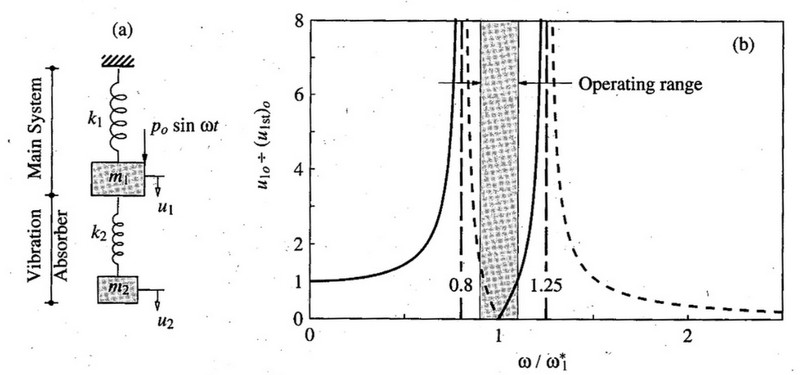
\includegraphics[width=4in]{figure/double}
	\end{figure}
	

\subsubsection{主动控制}
结构主动控制利用外界功能,在结构受风荷载、地震荷载等情况下受激励振动的过程中,根据外界激励信息和结构的响应,通过施加控制力,迅速改变结构在外界激励下的响应,从而控制结构振动。

主动控制系统可以分为主动质量阻尼系统(Active Mass Drive, AMD)、主动拉索系统ATS(Active Tendon System, ATS)、主动斜撑系统(Active Brace System, ABS)等。主动控制系统的工作模式可概述如下:传感器检测结构的动力响应和外部激励,将检测的信息传入计算机内,计算机根据给定的算法计算出控制力的大小,最后由AMD控制系统是主动控制系统的代表。1989年,日本东京建成世界上第一座采用AMD系统的大楼——Kyobasi Seiwa大厦\cite{T.KoboriN.KoshikaN.Yamada1991}。

随着控制算法的进步与计算机处理大规模实时数据能力的提升,主动控制系统的理论体系日趋完善,且控制效果十分出色,然而其大规模应用仍受到一些现实条件的制约:
\begin{enumerate}[leftmargin=*,labelindent=16pt,label=\bfseries \arabic*.]
	\item 严重依赖外界供能。主动控制系统完全依赖外界巨大的电能供应控制结构响应,在地震、风灾等极端条件下,电网安全难以保证,主动控制系统可能完全失效,而这恰恰是最需要结构控制的时候;
	\item 作动器吨位大,占据宝贵的建筑空间\cite{lou2013};
	\item 造价和运行维护成本高昂。
\end{enumerate}

\subsubsection{半主动控制}
结构振动的半主动控制是一种振动系统的参数控制技术,它根据系统输入的变化和对系统输出的要求,实时调节系统中元件的刚度、惯性或阻尼特性,从而改变结构的动力性能,达到控制结构振动的目的。

与被动控制系统相比,半主动控制系统的调节精度和控制范围远高于前者,对于控制建筑结构中随机性较大的地震动、风震有着良好的适应性。

半主动控制系统利用与结构的相对运动,只能向结构施加与其运动方向相反的控制力,无法实现完全主动的控制力,并且在控制精度和效果上不如主动控制系统;但是,半主动控制系统的作动器相较于主动控制系统而言成本较低,体积与重量也更易于被接受;此外,自供能的半主动控制系统利用结构往复振动产生的动能,对外界的能量输入依赖较低,克服了主动控制系统的能源问题。

综合以上论述,可以看到,半主动控制系统兼具了控制效果良好、设备简单经济的特点。

常见的半主动控制系统有:
\begin{enumerate}[leftmargin=*,labelindent=16pt,label=\bfseries \arabic*.]
	\item 主动调谐质量阻尼系统(Tuned Mass Damper, TMD),如台北101大厦的抗震体系;
	\item 可变刚度系统(Active Variable Stiffness, AVS),通过控制某些锁定装置,快速改变结构刚度,避开与外激励的共振频率,从而降低结构振幅响应。\cite{Lijing2006}显然,对于一般建筑,刚度设计值较大,为了能够提高控制效果,AVS的刚度要求较大,设计和经济意义上缺乏可行性。因此,AVS一般只应用于控制柔性结构;
	\item 可变阻尼系统(Active Viscosity System, AVS)通过调节元件中的阻尼大小,针对特定的外界激励提供相应的阻尼力,使其达到该激励下的理论最优控制力,工作模式接近主动控制系统,控制精度较高,且调节范围宽广且连续。然而,AVS控制系统中,阻尼大小一般只由速度控制,换言之,AVS无法控制结构位移;
\end{enumerate}

振动的半主动控制所涉及的关键技术是设计并实现可控减振环节与控制策略。\cite{Hu2001}可控减振环节可以具体分为可控弹性和惯性元件、可控阻尼器以及可控动力吸振器等几种类型。控制策略则以基于结构动力模型的控制策略为主,近年来,也出现了机器学习、人工神经元网络为代表的智能控制策略。

在后文中将提到的实验模型中,我们选择以可控阻尼器作为可控减震环节,控制策略则是基于模型的动力特性的算法。

\subsection{磁流变液与磁流变阻尼器}
\subsubsection{磁流变液(Magneto-Rheological Fluids(MRFs))}
磁流变液是研发于上世纪50年代的一种智能材料。典型的磁流变液由软磁性颗粒、粘滞流体和添加剂3种组分组成。在添加剂的作用下,软磁性颗粒与粘滞流体形成稳定均一的液态混合物,能够对外加磁场作出响应。

在没有外加磁场作用时,磁流变液的流变特性接近牛顿流体;在施加了外加磁场后,磁流变液则由牛顿流体转变为宾汉姆流体,即具有了一定的剪切屈服应力,并且,磁流变液的剪切屈服应力随着外加磁场的增强而连续增大,剪切屈服强度与外加磁场的磁感应强度大致呈正比例关系。

磁流变液在较大的磁感应强度变化范围内均呈现出上述的线性连续的“磁变特性”;同时,磁流变液对于外加磁场的响应时间达到毫米级,响应十分灵敏迅速\cite{Ali2015}。
此外,在一定的磁感应强度下,磁流变液达到剪切屈服应力后,磁流变液的滞回曲线十分饱满,具有良好的耗能性能,是一种理想的阻尼材料。

\subsubsection{磁流变阻尼器(MR Damper)}
磁流变阻尼器是以磁流变液作为阻尼材料的粘滞阻尼装置。

根据磁流变液在磁场作用下流变特性可控的特点,磁流变阻尼器可以根据结构的振动响应实时调整阻尼力,实现对结构振动的实时控制。可以看到,磁流变阻尼器具有阻尼力可调倍数高、响应时间短的特点\cite{Zhang2010}。

上面提到,主动控制系统中的作动器需要较大的能量输入,这一方面增加了控制系统的维护成本;另一方面也降低了系统在地震等环境下正常工作的可靠度。与之相比,磁流变阻尼器的驱动电压较低($10V$以内),借助结构的往复运动的能量,易于实现控制系统的自供能运转,提高了整个系统的可靠度。

与传统的阻尼材料相比,单位体积(或单位质量)的磁流变液能够提供更大的阻尼力,因此磁流变阻尼器具有较小质量与体积,节约了建筑空间,减轻了结构自重。


